\documentclass[11pt,a4paper]{report}
\usepackage[utf8]{inputenc}
\usepackage[french]{babel}
\usepackage[T1]{fontenc}
\usepackage{amsmath}
\usepackage{amsfonts}
\usepackage{amssymb}
\usepackage{xcolor}

\usepackage{geometry}
\geometry{hmargin=2.5cm,vmargin=1.5cm}
\usepackage{wasysym}
\usepackage{graphicx}

\author{Mathieu Sarrat}
\title{LP22 - Propriétés macroscopiques du ferromagnétisme}

\makeatletter
\renewcommand{\thesection}{\@arabic\c@section}
\makeatother


\begin{document}
\maketitle

\section*{Pré-requis et objectifs}
\begin{itemize}
	\item \'Electromagnétisme des milieux matériels (aimantation et équations de Maxwell)
	\item Loi de Faraday
	\item Inductance propre et inductance mutuelle
\end{itemize}

\subsubsection{Recommandations :}
\begin{itemize}
	\item Tracer en préparation un cycle d'hystérésis pour un matériau dur et pour un matériau mou.
\end{itemize}

\newpage
\section*{Introduction}

Les propriétés magnétiques de certains matériaux sont connues depuis l'Antiquité. Le mot magnétisme vient du nom de la ville de Magnésie, en Grèce, où l'on trouvait des pierres capables d'attirer le fer (les magnétites) : ces pierres d’aimant sont constituées d’oxyde de fer, $\text{Fe}_3\text{O}_4$. Le fer attiré par la magnétite possède alors temporairement les mêmes propriétés que la magnétite et peut aussi attirer certains matériaux.
\begin{figure}[h!]
\begin{center}
	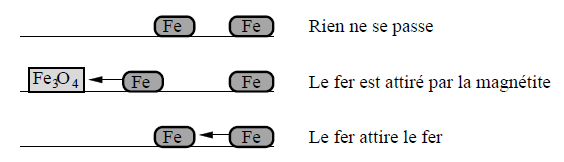
\includegraphics[scale = 0.50]{magnetite.png}
	\caption{Petite expérience de magnétisme.} 
	\label{fig:magnetite}
\end{center}
\end{figure}
Dans la vie quotidienne, on constate tous les jours la présence de corps possédant des propriétés magnétiques : aimants sur le réfrigérateur, aiguilles de boussoles, composants de transformateurs électriques, disques durs, ustensiles de cuisine.\\

Il existe plusieurs milieux possédant des propriétés magnétiques. On distingue notamment (liste non exhaustive) :
\begin{itemize}
	\item les milieux paramagnétiques : l'aimantation se fait dans le sens du champ magnétique 
	appliqué $\boldsymbol{B}_a$
	\item les milieux diamagnétiques : l'aimantation se fait dans le sens opposé à $\boldsymbol{B}_a$\\
	Dans ces deux cas, la réponse du matériau est de faible ampleur : l'aimantation est faible et 
	elle disparaît lorsqu'on retire $\boldsymbol{B}_a$ (il n'existe donc pas d'ordre magnétique 			spontané dans ces matériaux). 
	\item \textbf{les milieux ferromagnétiques} : l'aimantation se fait dans le sens
	de $\boldsymbol{B}_a$. Elle est \textbf{beaucoup plus importante} que dans le cas des matériaux 
	dia et paramagnétiques et persiste lorsqu'on retire le champ appliqué (phénomène de 					\textbf{rémanence}).\\
	
	\item Citons quelques \textbf{matériaux ferromagnétiques :}
	\begin{itemize}
		\item quelques rares \textbf{corps simples} : fer, cobalt, nickel, essentiellement,
		\item plusieurs \textbf{corps composés} : ferrites MO-$\text{Fe}_2\text{O}_3$ où 
			M désigne un métal divalent, oxydes métalliques (Cr$O_2$),
		\item \textbf{alliages} : Alnico, Ticonal, Alliages de Heusler, permalloy ...\\
	\end{itemize}
	
	\item Contrairement au paramagnétisme et au diamagnétisme, \textbf{le ferromagnétisme ne 				s'observe qu'avec des corps à l'état condensé}. Une molécule de dioxygène est paramagnétique, 			mais un atome de fer n'est pas ferromagnétique. Le ferromagnétisme résulte d'une interaction 			entre atomes ou molécules au sein d'une même structure cristalline. Les \textbf{alliages de 			Heusler}(ex : Cu$_2$MnAl ou Cu$_2$MnSn), en sont des exemples spectaculaires : pris séparément, 		Cu(s), Mn(s) ou Al(s) n'exhibent pas de comportement ferromagnétique, mais leur mélange oui.\\	
\end{itemize}
	
L'origine de ces propriétés ne peut pas s'expliquer dans le cadre de la physique classique (1920, Van Leuwen), aussi nous nous contenterons dans cette leçon d'une approche descriptive et macroscopique. Nous ne traiterons dans cette leçon que le cas du ferromagnétisme. Ses applications industrielles sont nombreuses. Nous commencerons par rappeler quelques notions d'électromagnétisme des milieux aimantés que nous appliquerons à un matériau ferromagnétique. On décrira ensuite les principales propriétés des matériaux ferromagnétiques, dont on mettra certaines en évidence à travers une expérience. On présentera enfin quelques applications concrètes et importantes du ferromagnétisme.

\newpage
\section{Rappels - aimantation de la matière}

Rappelons quelques notions d'électromagnétisme des milieux aimantés. Aller vite, toute la première partie ne doit pas dépasser 10 minutes.

\subsection{Aimantation d'un matériau}

L'application d'un champ magnétique à un milieu entraîne une réaction : il s'aimante. Un élément de volume de taille mésoscopique (suffisamment grande pour contenir un très grand nombre de particules, mais suffisamment petite devant les dimensions de l'aimant) porte alors un moment magnétique élémentaire $d\bold{\mathcal{M}}$ proportionnel à son volume $d\mathcal{V}$, tel que
\begin{equation}
	d\bold{\mathcal{M}} = \bold{M} \; d\mathcal{V}.
\end{equation}
où $\bold{M}$, l'\textbf{aimantation volumique} (ou aimantation) correspond à la densité volumique de moment magnétique, mesurée en $\text{A}.\text{m}^{-1}$.\\

On peut, selon l'idée d'Ampère (1821), attribuer l'origine de l'aimantation à l'existence de boucles de courant microscopiques. On associe donc à cette aimantation une densité volumique de courants d'aimantation telle que
\begin{equation}
	\bold{J}_\text{a} = \textbf{rot}\;\bold{M}.
\end{equation}
On sait que ces boucles de courant n'ont pas de réalité physique, et l'interprétation du magnétisme repose aujourd'hui sur un modèle quantique.\\

Insistons sur le fait que $\bold{M}$ et $\bold{J}_\text{a}$ sont des grandeurs définies à l'échelle mésoscopique, et donc des moyennes. Elles ne représentent pas une réalité microscopique, il s'agît d'une modélisation.

\subsection{Excitation magnétique}

On suppose que le milieu n'est pas polarisé, et qu'on travaille à suffisamment basse fréquence pour négliger le courant de déplacement dans l'équation de Maxwell-Ampère, que l'on peut alors réécrire :
\begin{equation}
	\textbf{rot}\;\bold{B} = \mu_0 \bold{J}.
\end{equation}

La densité volumique de courant $\bold{J}$ comporte plusieurs contributions :
\begin{equation}
	\bold{J} = \bold{J}_\text{int} + \bold{J_\text{ext}} 
	= \textbf{rot}\;\bold{M} + \bold{J}_m + \bold{J_\text{ext}}
\end{equation}
\begin{itemize}
	\item $\textbf{rot}\;\bold{M}$ est la densité de courant d'aimantation, introduite au paragraphe précédent,
	\item $\bold{J}_m$ est la densité de courants libres, qui peut exister si le milieu aimanté est un circuit fermé (milieu non-simplement connexe ; en régime stationnaire, c'est la densité de courant à l'origine de la valeur d'intensité mesurée par un ampèremètre).
	\item $\bold{J_\text{ext}}$ est la densité de courants libres situés hors du système étudié.\\
\end{itemize}

En injectant ces termes dans l'équation d'Ampère, puis en divisant par $mu_0$, on obtient :
\begin{equation}
	\textbf{rot}\;\bold{H} = \bold{J}_m + \bold{J_\text{ext}}.
\end{equation}
où on a défini le \textbf{champ d'excitation magnétique} noté $\bold{H}$, comme
\begin{equation}
	\boxed{\bold{H} \equiv \frac{\bold{B}}{\mu_0} - \bold{M}} \quad\text{ou encore}\quad 
	\bold{B} = \mu_0\left(\bold{H} + \bold{M}\right).
\end{equation}

Cette écriture est pratique d'un point de vue expérimental car les densités $\bold{J}_m$ et $\bold{J_\text{ext}}$ sont contrôlables ou mesurables par l'expérimentateur alors que $\textbf{rot}\;\bold{M}$ ne l'est pas. On établit un lien direct entre la cause (les courants appliqués par l'expérimentateur), et la conséquence (l'excitation magnétique du matériau). C'est pour cela que nous utiliserons préférentiellement $\bold{H}$ à $\bold{B}$ dans la suite de ce cours.\\

\newpage
La seconde relation permet d'interpréter le champ magnétique dans le matériau comme la somme de deux termes :
\begin{itemize}
	\item un champ magnétique dû aux courants extérieurs au système 
	\begin{equation}
		\bold{B}_\text{ext} = \mu_0 \bold{H}
	\end{equation}
	et donc responsable d'une excitation magnétique du système;
	\item cette excitation conduit à l'aimantation du matériau, et à un champ magnétique 
	résultant de celle-ci
	\begin{equation}
		\bold{B}_\text{aim} = \mu_0 \bold{M}.
	\end{equation}
\end{itemize}

\subsubsection{Relations de passage : (voir Pérez chapitre 23)}
\begin{equation}
	\bold{n}_{12}\cdot\left(\bold{B}_2 - \bold{B}_1\right) = 0
\end{equation}
\begin{equation}
	\bold{n}_{12}\times\left(\bold{H}_2 - \bold{H}_1\right) = 0
\end{equation}
où $\bold{J}_{m,s}$ désigne une éventuelle densité surfacique de courants libres (donc de courants de conduction).

\subsection{Susceptibilité magnétique}

Il reste à modéliser le lien entre l'excitation magnétique et l'aimantation du matériau, c'est à dire à \textbf{modéliser la réponse} du matériau. On introduit pour cela la notion de \textbf{susceptibilité magnétique} :
\begin{equation}
	\bold{M} = \chi^* \bold{H}.
\end{equation}
On a alors
\begin{equation}
	\bold{B} = \mu_0 \left(1 + \chi^* \right)\bold{H}
\end{equation}
et on définit la perméabilité magnétique relative du matériau
\begin{equation}
	\boxed{\mu_r \equiv 1 + \chi^*}
\end{equation}
et sa perméabilité absolue
\begin{equation}
	\boxed{\mu \equiv \mu_0\mu_r},
\end{equation}
de sorte que
\begin{equation}
	\boxed{\bold{B} = \mu\bold{H}}.
\end{equation}

La susceptibilité $\chi^*$ est positive pour un matériau paramagnétique (aimantation dans le sens du champ magnétique total), négative pour un matériau diamagnétique (aimantation dans le sens contraire au champ total). La valeur de cette grandeur est généralement très faible : cuivre (diamagnétique) $\chi^* \simeq - 10^{-6}$, eau (diamagnétique) $\chi^* \simeq - 10^{-5}$, oxygène liquide (paramagnétique) $\chi^* \simeq 10^{-3}$.\\

Un matériau est dit linéaire si la relation entre $\bold{B}$ et $\bold{H}$ est linéaire, ce qui implique que $\mu_r$ (et donc $\chi^*$) ne dépende pas de $\bold{H}$. Ce n'est pas le cas des milieux \textbf{ferromagnétiques qui sont non linéaires}, comme nous allons le voir dans un instant. La relation constitutive du matériau s'écrira
\begin{equation}
	\bold{M} = \chi^*(\bold{H}) \bold{H},
\end{equation}
la susceptibilité magnétique étant désormais une fonction de $\bold{H}$

\subsection{Lois fondamentales de l'électrotechnique}

\subsubsection{Théorème d'Ampère}

Forme globale du théorème d'Ampère : on intègre sur la surface $S$ du contour $\mathcal{C}$ :
\begin{equation}
	\iint_S \textbf{rot}\bold{H}\cdot\bold{n}dS = \oint_\mathcal{C} \bold{H}\cdot d\bold{r} = \iint_S \left(\bold{J}_\text{m}+\bold{J}_\text{ext}\right)\cdot\bold{n}dS = I_m + I_\text{ext},
\end{equation}
d'où
\begin{equation}
	\boxed{\oint_\mathcal{C} \bold{H}\cdot d\bold{r} = I_m + I_\text{ext}}.
\end{equation}
Seuls les courants circulant à travers $S$ sont pris en compte dans le calcul. La circulation de $\bold{H}$ est calculée le long du contour $\mathcal{C}$ qui délimite la surface $S$.

\begin{figure}[h!]
\begin{center}
	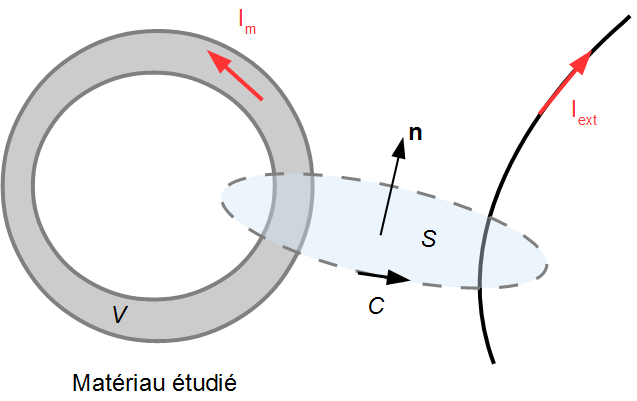
\includegraphics[scale = 0.30]{ampere_theo.png}
	\caption{Démonstration du théorème d'Ampère.} 
	\label{fig:ampere_theo}
\end{center}
\end{figure}

\subsubsection{Loi de Faraday}

La loi de Faraday s'établit en intégrant l'équation de Maxwell-Faraday sur une surface s'appuyant sur un contour fermé $\mathcal{C}$. On suppose un contour indéformable et immobile, de sorte que l'intégration est immédiate et conduit à la Loi de Faraday
\begin{equation}
	\boxed{e = - \frac{d\Phi}{dt}} = \oint_\mathcal{C} \bold{E}\cdot\bold{d\ell},
\end{equation}
où $e$ est la force électromotrice générée dans le circuit étudié.

\newpage
\section{Aimantation et propriétés d'un matériau ferromagnétique}

\subsection{Modèle du circuit magnétique torique}
On suppose un circuit ferromagnétique torique de section carrée (de surface $A_e$ et de côté $a$), symétrique par révolution autour de l'axe $Oz$. On place un enroulement de N spires, parcourues par un courant électrique d'intensité $I$ autour de la circonférence de ce tore. On souhaite déterminer le champ magnétique en un point M de l'espace. Tout plan $(\bold{OM},Oz)$ est plan de symétrie de la distribution des courants, par ailleurs invariante par rotation autour de l'axe Oz. Aussi
\begin{equation}
	\bold{B} = B(r) \bold{e}_\theta, \quad\text{d'où}\quad \bold{H} 
	= \frac{B}{\mu_0 \mu_r} = H(r) \bold{e}_\theta.
\end{equation}
On applique le théorème d'Ampère sur un contour circulaire $\mathcal{C}$ de rayon $r$ et de centre 0 
\begin{equation}
	\oint_\mathcal{C} \bold{H}\cdot\bold{d\ell} = NI_\text{ext} \equiv N I,
\end{equation}
pour simplifier les notations, d'où
\begin{equation}
	\bold{B} = \mu_0\mu_r \frac{NI}{2\pi r}\bold{e}_\theta.
\end{equation}

On calcule le flux de ce champ à travers la section carrée du tore, en supposant que le champ magnétique ne dépend pas de $z$ :
\begin{equation}
	\Phi = \iint_{A_e}\bold{B}\cdot\bold{dS} 
	= \int_{R - \frac{a}{2}}^{R+\frac{a}{2}} \mu_0\mu_r \frac{NI}{2\pi r}a\;dr
	= \mu_0\mu_r \frac{NIa}{2\pi}\text{ln}\left( \frac{R+a/2}{R-a/2}\right).
\end{equation}

Si $a \ll R$, alors
\begin{equation}
	\Phi = \mu_0 \mu_r \frac{NIa^2}{2\pi R}.
\end{equation}
Cela revient à assimiler un champ magnétique homogène dans le circuit magnétique, égal à la valeur qu'il prend le long de la ligne de champ moyenne, de rayon R :
\begin{equation}
	B = \mu_0\mu_r \frac{NI}{2\pi R}.
\end{equation}

\subsection{Courbe de première aimantation}
La connaissance de $\mu(H)$ est nécessaire pour caractériser le matériau : aussi, nous allons tracer la courbe $B(H)$. On souhaite donc mesurer :
\begin{itemize}
	\item le champ magnétique $\bold{B}$ dans le circuit magnétique,
	\item l'excitation magnétique $\bold{H}$.
\end{itemize}
L'aimantation pourra être déduite par la relation
\begin{equation}
	\bold{B} = \mu_0\left(\bold{H} + \bold{M}\right) = \mu(H)\bold{H}
\end{equation}
et on pourra aussi calculer la perméabilité magnétique absolue
\begin{equation}
	\mu = \frac{\bold{B}}{\bold{H}}.
\end{equation}

\subsubsection{Présentation du montage}
Pour tracer cette courbe, nous allons utiliser le montage suivant : deux solénoïdes non reliés électriquement entre eux sont enroulés autour d'un circuit magnétique rectangulaire, de section carrée.

\begin{figure}[h!]
\begin{center}
	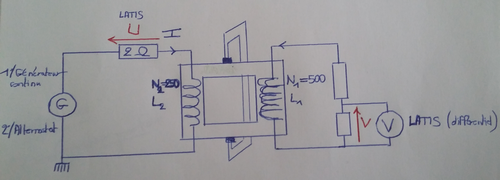
\includegraphics[scale = 0.70]{montage.png}
	\caption{Montage d'aimantation d'un circuit ferromagnétique. Erreur sur les indices de $N$, mais 		pas sur les valeurs.} 
	\label{fig:montage}
\end{center}
\end{figure}

\begin{itemize}
	\item Le premier solénoïde ($N_1 = 250$) est connecté en série avec un rhéostat, réglé sur $R = 2$ Ohms (en réalité, on choisit cette valeur pour utiliser la pleine échelle de la carte d'acquisition) et l'ensemble est alimenté par un générateur de courant délivrant une intensité $I$ contrôlable. On règle l'intensité maximale de sorte à ne pas dépasser la valeur maximale supportée par les composants (notamment la bobine). Le courant $I$ est calculé à partir de la mesure de la tension aux bornes du rhéostat. Sa connaissance nous permet de déterminer $H$ : on suppose pour cela que les lignes de champ magnétique sont parfaitement canalisées par le milieu ferromagnétique, et nous allons légèrement modifier les résultats du modèle du circuit torique présenté plus haut. Ainsi
\begin{equation}
	H = \frac{N_1 I}{\ell} = \frac{N_1 U}{R\ell},
\end{equation}
où $\ell$ est la longueur de la ligne de champ moyenne. On a supposé que $N_2 i_2$, où $i_2$ désigne le courant circulant dans le second enroulement, est négligeable devant $N_1 I$.\\

	\item Le second solénoïde ($N_2 = 500$) est connecté en série à deux résistances $R_1$ et $R_2$. On prélève la tension aux bornes de la résistance la plus faible $R_2$ (pont diviseur de tension) grâce à une carte d'acquisition (et le logiciel Latis Pro) via deux entrées fonctionnant en mode différentiel. Si on néglige la résistance interne du solénoïde, la tension à ses bornes est égale à l'opposé de la force électromotrice dans la bobine, donnée par la loi de Faraday :
\begin{equation}
	V = \frac{R_2}{R_1 + R_2} \frac{d\Phi}{dt}
\end{equation}
où $\Phi$ désigne le flux du champ magnétique total régnant dans le milieu ferromagnétique à travers les $N_2$ spires du solénoïde :
\begin{equation}
	\Phi(t) = N_2 A_e B(t),
\end{equation}
$A_e$ désignant la section carrée du tore. La carte d'acquisition mesure $V$, on peut remonter à $B(t)$ par intégration en utilisant le module de calcul de Latis Pro :
\begin{equation}
	B = \frac{R_2 + R_1}{R_2 N_2 A_e}\;\text{Integ}(EA26_D;Temps;).
\end{equation}
\end{itemize}

On part de $I = 0$, on monte jusqu'à $I_\text{max}$ puis on fait décroitre $I$ jusqu'à 0. On obtient ainsi trois résultats :
\begin{itemize}
	\item la \textbf{courbe de première aimantation :} on montre les courbes $B(H)$ 
	et $M(H) = B(H)/\mu_0 - H = f(H)$, le matériau étant initialement non aimanté et obtenue en faisant 	croître $I$ (essayer d'atteindre la saturation). 
	
	\begin{itemize}
		\item \`A \textbf{faible excitation} magnétique, la courbe $B(H)$ est parabolique 
		(domaine de Rayleigh), impliquant une relation de proportionnalité entre $\mu_r$ et $H$.
		\item \`A \textbf{forte excitation}, le champ magnétique augmente moins vite et l'aimantation 			sature. On peut alors mesurer \textbf{l'aimantation à saturation} $M_\text{sat}$ 
		(en A/M) ou $\mu_0 M_s$ en Tesla;
	\end{itemize}
	
	\begin{figure}[h!]
	\begin{center}
		\begin{tabular}{|c|c|c|c|}
		\hline
		Matériaux & Fer & Cobalt & Nickel \\
		\hline
		$\mu_0\;M_s(T)$ & 2.19 & 1.8 & 0.64 \\
		\hline
		\end{tabular}	
	\end{center}
	\end{figure}
	
	\item on met en évidence l'existence d'un \textbf{champ magnétique rémanent} $B_r$ important sur la 	courbe B(H), lorsqu'au retour $I =$ 0 (et donc $H = 0$). On peut mesurer $B_r$;
	
	\item on trace $\mu(H)$ : cette courbe présente un maximum, et on remarque que la valeur de $\mu$ 		dépend fortement de l'excitation magnétique.
	\begin{figure}[h!]
	\begin{center}
		\begin{tabular}{|c|c|c|c|c|}
		\hline
		Matériaux & fer pur & mumétal & permalloy & acier trempé \\
		\hline
		$(\mu_r)_\text{max}$ & $5\times10^{5}$ & $3\times10^{4}$ & $5\times10^{5}$ & 98\\
		\hline
		\end{tabular}	
	\end{center}
	\end{figure}
\end{itemize}

\subsection{Cycle d'hystérésis}

\subsubsection{Mise en évidence}
On remplace le générateur de courant continu par un alternostat fonctionnant à 50 Hz et délivrant tension et courant alternatifs. On utilise une pince ampèremétrique pour mesurer le courant $i$ (on met une lettre minuscule puisqu'on mesure un courant alternatif). Faire le zéro sur la pince ampèremétrique pour que le cycle soit bien centré \textcolor{red}{(ou faire tout bêtement l'acquisition de tension aux bornes du rhéostat, car la pince ampèremétrique donne probablement un courant efficace, là où on veut la valeur instantanée)}.

\subsubsection{Irréversibilité, non-linéarité}
En faisant l'acquisition sur 5 secondes, le diagramme B(H) prend l'allure d'un cycle. L'existence même de ce cycle implique l'irréversibilité (la transformation inverse ne passe pas par le même "chemin" dans l'espace des variables d'état) et la non-linéarité du processus d'aimantation (à une valeur de l'excitation correspond deux valeurs possibles de la réponse, i.e. du champ magnétique), ce que nous avons pu constater précédemment en réduisant progressivement le courant circulant dans le solénoïde primaire.

\subsubsection{Excitation coercitive et annulation de la rémanence}
L'intersection du cycle avec l'axe horizontal implique qu'il est nécessaire d'appliquer une excitation magnétique non-nulle pour annuler le champ magnétique dans le milieu. Cette excitation magnétique est appelée \textbf{excitation coercitive et est notée $H_c$. Tout comme celle du champ rémanent, sa valeur est une caractéristique du matériau ferromagnétique considéré.} Il est donc possible de désaimanter une substance possédant un champ rémanent.

\subsubsection{Matériaux durs et doux}
\textcolor{red}{Montrer les cycles pour les deux types de matériaux, réalisés en préparation.}\\

On appelle \textbf{matériaux magnétiques doux} ceux dans lesquels le champ coercitif est petit. La surface de leur cycle d'hystérésis principal est faible. Le permalloy ou le fer pur sont deux exemples de tels matériaux.\\

On appelle \textbf{matériaux magnétiques durs} ceux dans lesquels le champ coercitif est élevé. La surface de leur cycle d'hystérésis est importante. Le champ rémanent est important, d'où leur unique application : la fabrication d'aimants permanents.\\

C'est la valeur de l'excitation coercitive $H_c$ qui détermine le caractère doux ou dur d'un matériau ferromagnétique. En pratique, on admet :\\
\begin{itemize}
	\item $H_c < 100$ A/m correspond à un matériau doux,
	\item $H_c > 100$ A/m correspond à un matériau dur.
\end{itemize}

\newpage
\subsubsection{Pertes fer}

Toute variation du champ magnétique dans un matériau magnétique provoque à l'intérieur de celui-ci une dissipation d'énergie, le plus souvent sous forme de chaleur. On parle de pertes magnétiques ou de \textbf{pertes fer} et on distingue parmi celles-ci :
\begin{itemize}
	\item les pertes par hystérésis,
	\item les pertes par courant de Foucault.\\
\end{itemize}

Les pertes par hystérésis correspondent au travail nécessaire pour parcourir lentement le diagramme B(H).\\

S'ajoutent à elles les pertes par courant de Foucault : ces pertes résultent de l'effet Joule lié aux courants créés dans le circuit magnétique s'il est conducteur. Il est difficile de séparer ces pertes dans un cycle dynamique comme celui que nous venons de réaliser, aussi nous évaluerons le total.\\

En négligeant l'effet Joule lié à la résistance interne du solénoïde primaire, la puissance consommée au primaire vaut
\begin{equation}
	P_1 = u_1(t) i_1(t) = - e_1(t) i_1(t) = N_1\frac{d\Phi_1}{dt}i(t),
\end{equation}
or, en supposant négligeable l'excitation générée par le secondaire ($N_1 i_1  >> N_2 i_2$), on peut écrire
\begin{equation}
	i_1(t) = \frac{\ell H(t)}{N_1}
\end{equation}
et
\begin{equation}
	N_1 \frac{d\Phi}{dt} = N_1 A_e \frac{dB}{dt},
\end{equation}
d'où
\begin{equation}
	P_1(t) = \ell A_e H(t) \frac{dB}{dt} \simeq \mathcal{V}_e H(t) \frac{dB}{dt}
\end{equation}
où $\mathcal{V}_e$ désigne le volume du matériau ferromagnétique. On moyenne sur une période $T = 1/f$ (du courant produit par l'alternostat) :
\begin{equation}
	\boxed{\left\langle P_1 \right\rangle = \mathcal{V}_e f \int_0^T HdB}
\end{equation}
où la quantité représentée par l'intégrale n'est rien d'autre que l'aire du cycle d'hystérésis. \textcolor{red}{On calcule l'aire du cycle grâce à Latis Pro pour remonter à la puissance moyenne perdue sur un cycle, à la fréquence de 50 Hz.}\\

Les pertes fer augmentent donc avec la fréquence de l'excitation magnétique du matériau ferromagnétique. \textit{L'aire du cycle d'hystérésis augmente aussi avec la fréquence, mais on ne peut pas expliquer cet élargissement du cycle par les seuls courants de Foucault.}\\

\newpage
\section{Applications}

Nous allons maintenant détailler quelques applications de matériaux ferromagnétiques. Nous avons distingué deux grandes catégories de matériaux ferromagnétiques, les matériaux doux et les matériaux durs. On les distingue par la valeur de leur excitation coercitive $H_c$.\\

Celle-ci est élevée pour les ferromagnétiques durs : il est donc difficile de désaimanter ces matériaux qui sont donc utilisés comme aimants permanents. Les applications de tels aimants sont nombreuses, puisqu'on les retrouve dans les machines électriques tournantes (moteurs, générateurs), dans les écouteurs téléphoniques et haut-parleurs ou encore dans des supports d'enregistrement : bandes et disques magnétiques.\\

Les pertes fer étant d'autant plus importantes que l'aire du cycle d'hystérésis est grande : les matériaux durs sont donc ceux pour lesquels les pertes seront les plus élevées lors d'une utilisation en fonctionnement dynamique. On leur préfèrera donc des matériaux doux dès lors qu'un fonctionnement dynamique sera souhaité. C'est par exemple le cas des transformateurs électriques.

\subsection{Transformateur parfait}

Un transformateur électrique permet de modifier les valeurs de tension et d'intensité du courant délivrées par une source d'énergie électrique alternative : on obtient un signal de tension et de courant de valeurs différentes, mais de même fréquence et de même forme. Ceci est très important dans la distribution du courant électrique : le transport sur de longues distances étant moins coûteux lorsque la tension utilisée est plus grande, des transformateurs élèvent jusqu'à 400 kV la tension alternative de 25 kV délivrée en sortie de centrale nucléaire. Pour une utilisation domestique, il faut réaliser l'opération inverse et ramener la tension à 220 V. On utilise plusieurs échelons de transformation pour cela.\\

Dans un transformateur statique, l'énergie est transférée d'un enroulement (une bobine de $N_1$ spires, souvent en cuivre) dit \textbf{primaire} à l'enroulement dit \textbf{secondaire} (une autre bobine en cuivre, mais de $N_2$ spires) par l'intermédiaire du \textbf{circuit magnétique} que constitue la carcasse du transformateur. Les deux \textbf{enroulements sont couplés par induction mutuelle} et ne sont pas reliés électriquement.

\begin{figure}[h!]
	\begin{center}
		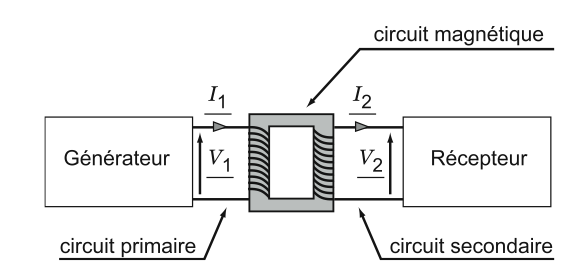
\includegraphics[scale = 0.4]{transfo.png}
		\caption{Représentation simplifiée d'un transformateur électrique} 
		\label{fig:transfo}
	\end{center}
\end{figure}

Le rendement de l'installation et d'autant meilleur que le couplage entre les circuits est serré, c'est à dire que la plus grande partie des lignes de champ magnétique sortant d'un enroulement entre dans le second. Pour améliorer ce rendement, le circuit magnétique est conçu en matériau ferromagnétique (souvent un fer doux). On retrouve en quelque sorte le montage que nous avons utilisé pour étudier les propriétés du circuit magnétique.\\

Si on reprend le modèle du circuit magnétique torique, l'excitation magnétique liée aux courants $i_1$ et $i_2$ circulant dans les enroulements s'écrit
\begin{equation}
	H = \frac{N_1 i_1 + N_2 i_2}{2 \pi R}.
\end{equation}

Le modèle du transformateur parfait repose sur trois grandes hypothèses :
\begin{itemize}
	\item le circuit magnétique est supposé linéaire, homogène et isotrope. La linéarité suppose une 		excitation magnétique suffisamment faible, ce qui est assuré si on prend une perméabilité 				magnétique relative infinie : le champ magnétique étant fini, cela impose une excitation magnétique 	nulle dans le circuits;
	\item les lignes de champ sont parfaitement canalisées par le ferromagnétique : il n'y a pas de 		fuites magnétiques;
	\item les enroulements conducteurs sont des conducteurs parfaits : il n'y a pas de pertes Joule.\\
\end{itemize}

Comme $H = 0$,
\begin{equation}
	\boxed{i_1 = -\frac{N_2}{N_1}i_2 = - m i_2}\quad\text{où}\quad
	m \equiv \frac{N_2}{N_1}\quad\text{est le \textbf{rapport de transformation}.}	
\end{equation}
Compte tenu des forces électromotrices d'induction, chaque enroulement présente une tension à ses bornes
\begin{equation}
	v_1 = -e_1 = N_1\frac{d\Phi}{dt}\quad\text{et}\quad
	v_2 = -e_2 = N_2\frac{d\Phi}{dt}
\end{equation}
où $\Phi$ désigne le flux total du champ magnétique à travers la section droite du matériau magnétique. On a ainsi
\begin{equation}
	\frac{v_2}{v_1} = \frac{N_2}{N_1} = m.
\end{equation}

Par ailleurs, on peut écrire
\begin{equation}
	N_1\Phi = L_1 i_1 + M i_2 \quad\text{et}\quad N_2\Phi = L_2 i_2 + M i_1,
\end{equation}
où $L_1$ et $L_2$ sont les inductances propres des deux solénoïdes et $M$ l'inductance mutuelle du système, d'où
\begin{equation}
	v_1 = L_1 \frac{d i_1}{dt} + M \frac{d i_2}{dt} 
	\quad\text{et}\quad
	v_2 = L_2 \frac{d i_2}{dt} + M \frac{d i_1}{dt}.
\end{equation}

En réalité, il existe plusieurs sources de pertes dans un transformateur. Voici les principales :
\begin{itemize}
	\item \textbf{les pertes fer :} ce sont les pertes dans le circuit magnétique. Leur origine physique est double : les courants induits (courants de Foucault) générés dans le noyau de fer doux et les pertes par hystérésis. On minimise ces pertes en choisissant un matériau ferromagnétique doux (réduction des pertes par hystérésis, le cycle étant moins large) et en privilégiant un circuit magnétique constitué de tôles isolées électriquement les unes des autres (feuilletage pour réduire les pertes par courants de Foucault). Le circuit magnétique est constitué de fines tôles de fer doux empilées les unes sur les autres, un vernis isolant permettant de limiter la circulation du courant d'une tôle à l'autre. Les pertes par courants de Foucault étant proportionnelles au volume du matériau ferromagnétique, ce feuilletage permet de les réduire;
	\item \textbf{les pertes cuivre :} ce sont les pertes par effet Joule dans les enroulements, qui possèdent eux aussi une résistance interne;
	\item \textbf{les fuites de flux :} on considère dans notre modèle que le flux est entièrement canalisé par le circuit magnétique, ce qui n'est pas le cas. Le flux circule donc partiellement hors du noyau.
\end{itemize}

\subsection{Disque dur}

Le disque dur est l'un des organes centraux de l'ordinateur : il stocke et conserve les données.

\subsubsection{Principe d'écriture}
Ensemble de plateaux (en verre ou en aluminium) recouverts d'un matériau ferromagnétique (alliage d'oxyde de fer, de nickel et de cobalt), initialement non aimanté.

On produit un champ magnétique de direction constante mais dont on peut choisir le sens (un sens correspond à 0, l'autre sens correspond à 1). Ainsi on aimante localement (domaine de Weiss) le matériau en fonction de l'information à coder.\\

Le champ magnétique est produit par une bobine dans laquelle on fait circuler un courant électrique. Changer le sens du courant permet de changer le sens du champ magnétique produit. On introduit un ferromagnétique doux dans la bobine pour amplifier le champ : il s'aimante et produit un champ 
\begin{equation}
	\bold{B}_\text{aim} = \mu_0 \bold{M}
\end{equation}
s'ajoutant au champ excitateur produit par la bobine,
\begin{equation}
	\bold{B}_\text{ext} = \mu_0 \bold{H}.
\end{equation}

\subsubsection{Principe de lecture}
Anciennement : le passage de la tête de lecture au-dessus d'une zone aimantée provoque un courant induit dans la bobine servant à l'écriture. Ce courant étant faible, la taille d'une zone d'aimantation  homogène (qu'on appelle domaine de Weiss) doit être assez grande. Cela limite la quantité d'informations qu'on peut stocker.\\

Aujourd'hui, on tire profit de la capacité qu'ont certains matériaux à voir varier leur résistance électrique en fonction du champ magnétique dans lequel ils sont plongés (la mesure d'une résistance est une mesure plus simple à réaliser). C'est l'effet de \textbf{magnétorésistance géante}, dont la découverte a valu le prix Nobel en 2007 à Albert Fert, et dont l'étude dépasse très largement le cadre de cette leçon.

\section*{Conclusion}

Importance des corps ferromagnétiques en électricité appliquée (finalité industrielle) : aimants artificiels, machines électriques, transformateurs...\\ 

On s'est limités à une approche macroscopique descriptive et classique. Expérimentalement (microscopie), on observe des \textbf{domaines de Weiss}, séparés par des parois. Au sein d'un domaine, l'aimantation est uniforme, mais elle varie d'un domaine à l'autre. Lorsqu'on applique un champ magnétique, les domaines dont l'aimantation est colinéaire au champ appliqué augmentent de volume jusqu'à ce qu'il n'y ait plus qu'un seul domaine. Nécessité d'une description quantique (prise en compte du spin des atomes, et de l'interaction entre spins).\\

Température de Curie : au-delà d'une certaine température, le matériau subit une transition de phase (d'ordre deux). Il passe de l'état ferromagnétique à l'état paramagnétique. Un aimant permanent chauffé au-delà de sa température de Curie est perd ses propriétés magnétiques (plus de champ rémanent).

\section*{Annexes}
\subsection*{Autre définition de la susceptibilité magnétique}

Dans un milieu linéaire, la relation entre $\bold{M}$ et $\bold{B}$ (le champ magnétique total : appliqué $+$ produit par le milieu) est une relation de proportionnalité :
\begin{equation}
	\bold{M} = \chi_m \frac{\bold{B}}{\mu_0} \quad\text{auquel cas}\quad
	\chi^* = \frac{\chi_m}{1-\chi_m},
\end{equation}
Dans un matériau \textbf{linéaire, homogène et isotrope}, la susceptibilité magnétique est un scalaire de valeur constante en tout point du matériau. On a dans ce cas
\begin{equation}
	\bold{H} = \frac{\bold{B}}{\mu_0} - \bold{M} = \left(1-\chi_m\right)\frac{\bold{B}}{\mu_0} \equiv \frac{\bold{B}}{\mu_0\mu_r}\quad\text{avec}\quad 	\mu_r = \frac{1}{1-\chi_m},
\end{equation}
la \textbf{perméabilité relative} du matériau. Le produit $\mu = \mu_0\mu_r$ est appelé perméabilité absolue du matériau.

\subsection*{Propriétés du ferromagnétisme (facultatif ou manip d'intro)}

Mettons tout d'abord en évidence quelques propriétés des matériaux ferromagnétiques.

\subsubsection{Aimantation, rémanence}
\begin{itemize}
	\item \textcolor{red}{\textbf{Manip :}}
	\begin{itemize}
		\item Connecter un solénoïde à un générateur électrique éteint.
		\item Allumer le générateur (courant électrique constant) et mesurer le champ magnétique au 				moyen d'un teslamètre, après avoir fait le zéro de celui-ci.
		\item Approcher du solénoïde un noyau de fer (non-aimanté). Mesurer le champ magnétique et 					constater l'augmentation du champ.
		\item Constater l'attraction entre le noyau et le solénoïde.
		\item Couper l'alimentation et mesurer le champ magnétique. Constater l'existence d'un champ 				rémanent.\\
	\end{itemize}
	
	\item \textbf{Interprétation : }
	\begin{itemize}
		\item Le noyau de fer est attiré par le solénoïde et s'immobilise là où le champ est 
			le plus intense. Il existe donc une force exercée par le champ magnétique sur l'aimant.
		\item Le champ magnétique au voisinage de l'ensemble est plus intense après introduction du 				noyau : matériau aimanté produisant un champ magnétique s'ajoutant au champ initial.
		\item En coupant le courant, un $B$ plus faible subsiste : aimant permanent et rémanence.\\
	\end{itemize}
\end{itemize}

\textbf{Comparaison avec le paramagnétisme :} les deux premiers résultats sont en nature analogues à ceux obtenus pour une substance paramagnétique, mais ils sont plus forts. L'augmentation relative du champ magnétique avec un matériau paramagnétique est au mieux de $10^{-3}$ \textcolor{red}{Comparer avec l'augmentation de B mesurée}. \textbf{La rémanence n'est pas constatée avec un matériau paramagnétique.}

\subsubsection{Température de Curie}	

Au-delà de $T_C$, le ferromagnétisme disparaît et le matériau se comporte comme un corps paramagnétique. Ce changement est associé à une transition de phase (du second ordre). Au-delà de la température de Curie :
\begin{equation}
	\boxed{\chi_m (T) = \frac{C}{T-T_C}}
\end{equation}
où $C$ est la constante de Curie. C'est la loi de Curie-Weiss.\\
		
\begin{figure}[h!]
	\begin{center}
	\begin{tabular}{|c|c|c|c|c|c|}
  	\hline
  	Matériaux & Cobalt & Fer  & Nickel & CrO2 & MnO–Fe$_2$O$_3$\\
 	\hline
  	$T_C$ (K) & 1388   & 1043 & 627    & 386  & 573 \\
  	\hline
	\end{tabular}
	\end{center}
	\caption{Quelques valeurs de $T_C$.}
\end{figure}
	
\end{document}